\section{ViSIT Metadaten und die Semantische Datenbank}\label{sec:semantics}

Brainstorm, things to write about:

\begin{itemize}
	\item theoretischer background: rdf daten, CIDOC, Vismo
	\item datenbank: infrastruktur (hosting, allgemeiner zugriff von aussen), drupal, wisski (allgemein), grundfunktionalität
	\item wisski: rdf daten, pfade, konfiguration
	\item REST API: allgemeine beschreibung
	\item zusatzfeatures: copy and paste, excel import
\end{itemize}

\subsection{Theoretische Grundlagen für die Semantische Datenbank}\label{sec:theoreticalBackground}

Dieses Unterkapitel gibt Einblicke in Teilbereiche des Semantic Webs, um eine theoretische Grundlage für die folgenden technischen Entwicklungen zu geben. Nachdem diese erläutert wurden, wird ebenfalls auf eine spezielle Ausprägung eines Metadatenmodells eingegangen, welches die Struktur für die im ViSIT Projekt verwendeten Metadaten vorgibt: das ViSIT Model \textbf{VisMo}.

Die hier angeführten Ausführungen beschränken sich jedoch nur auf jeweilige Grundlagen der Themenkomplexe, welche an manchen Stellen um weiterführende Informationen erweitert werden, wenn dies für den weiteren Verlauf von Nöten ist. Dennoch, falls angestrebt, verweisen wir für ein tieferes Verständnis auf weitere Fachliteratur, wie z.B. \cite{Hitzler-SemanticWeb-2007}.

\paragraph{Semantic Web und RDF Daten}

Das Semantic Web ist eine Art Erweiterung zum eigentlichen World Wide Web, wie wir es aktuell kennen. Dieses ist primär für Menschen ausgelegt, die durch Homepages browsen und dabei entsprechende Informationen durch betrachten und lesen der Homepages erlangen. Diese Informationen sind dadurch jedoch nur für Menschen vorhanden, Maschinen oder Computer können auf die Informationen nicht zugreifen, um mit den entsprechenden Daten arbeiten zu können. Genau hier setzt das Semantic Web an, welches Standardisierungen, Regeln und Prozesse vorgibt, um Homepages und Applikationen so anzupassen, dass eben genau eine (semi-) automatische Informationsverarbeitung für Maschinen möglich wird.
 
Eine dieser Standardisierungen ist das Resource Description Framework \textbf{RDF} \cite{Manola-RDFPrimer1.0-2004}, welches der de-facto Standart im Semantic Web ist, um Metadaten zu beschreiben. Daten in RDF werden als Graph modelliert und persistiert, welcher aus Knoten und Kanten besteht. Dabei entsteht eine Wissensbasis gefüllt an Informationen. Die Knoten sind hierbei die \q{Akteure}, also diejenigen Entitäten, Sachen, Objekte, Dinge etc., ausgehend vom jeweiligen Anwendungsfall, auf die sich die im Graphen enthaltenen Informationen beziehen (diese Dinge werden im Folgenden weiterhin als \q{Metadatenentität} bezeichnet). Die Kanten im Graphen beschreiben Beziehungen zwischen den gegebenen Knoten und Eigenschaften der Knoten. Weiterhin sind die Knoten und Kanten durch das Grundprinzip eines \textbf{Statements} verbunden, welches eine Kapselung einer elementaren Aussage darstellt. Das Statement ist, ähnlich dem deutschen Satzbau, immer bestehend aus drei Teilen:

\begin{description}
	\item[Subjekt] Die Metadatenentität repräsentiert als ein Knoten im Graphen, von der die Aussage - und damit das Prädikat - des Statements ausgeht.
	\item[Prädikat] Die Semantik oder die Bedeutung der Aussage.
	\item[Objekt] Zweierlei Konzepte können das Objekt des Statements bilden: ein weiterer Knoten im Graphen, um das Ziel der Aussage und damit des Prädikats, um eine Relation zwischen zwei Metadatenentitäten/Knoten darzustellen, oder ein fester Wert, um eine Eigenschaft einer Metadatenentitäten/eines Knotens zu charakterisieren.
\end{description}

Zur Verständlichkeit für die Thematik der Aussagen und Statements im Semantic Web Kontext, soll hier ein kurzes, erfundenes Beispiel erläutert werden. Folgende Aussagen bilden die Wissensbasis:

\begin{itemize}
	\item Peter ist vom Beruf Baumeister.
	\item Peter ist 40 Jahre alt.
	\item Peter war am Bau des Steinschlosses beteiligt.
	\item Das Steinschloss besteht aus Stein.
	\item Das Steinschloss ist 10 Jahre alt.
\end{itemize}

Wie oben beschrieben, bestehen die Aussagen jeweils aus Subjekt, Prädikat und Objekt. Als Subjekte agieren die beiden Metadatenentitäten \q{Peter} und das \q{Steinschloss}, während die Objekte der Aussagen der Beruf \q{Baumeister}, das Material \q{Stein}, zwei \q{Altersangaben}, sowie das \q{Steinschloss} selbst sind. Semantisch sind die Subjekte und Objekte über die Beziehungen bzw. Eigenschaften einer \q{Berufszuordnung}, zwei \q{Alterszuordnungen}, einer \q{Materialzuweisung} sowie der \q{Erbauung} eines Objekts verbunden.

Diese Aussagen können nun in einen Graphen zusammengefasst werden, dessen high-level Illustration in \autoref{fig:statements} zu sehen ist.

\begin{figure}[htb]
    \centering
    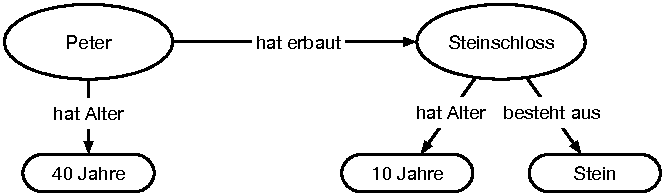
\includegraphics[width=\textwidth]{Figures/berndl/statements}
    \caption{\label{fig:statements} Informationen aus obigen Aussagen, kombiniert als Graph.}
\end{figure}

\paragraph{Linked Open Data Gedanke}

Ein weiterer Eckpfeiler des Semantic Web ist ein weiteres Konzept, das unter dem Namen \textbf{Linked Open Data - LOD} bekannt ist. Oft wird dieser Name ebenfalls für das Semantic Web selbst benutzt, die punktgenauen Definitionen überschneiden und ergänzen sich.

Einfach übersetzt zielt LOD auf öffentlich zugängliche Daten ab, die untereinander vernetzt und verlinkt sind. Somit soll es möglich sein, verteilte Datenbanken mit ihren eigenen entsprechenden Wissensbasen, miteinander zu verbinden, um so jedem Beteiligten mehr Informationen zur Verfügung zu stellen, da durch die Verlinkung einzelner Graphen ein großer Gesamtgraph entsteht. ...

\paragraph{Zwei Anwendungsfälle für RDF im Geschichtswissenschaftlichen Kontext}

blub

\paragraph{Das CIDOC CRM}

blub

\paragraph{Das ViSIT Model - VisMo}

blub

\subsection{Technische Details zur Semantischen Datenbank}\label{sec:technicalBackground}

infrastruktur, hosting, allgemeiner zugriff

zertifizierung, sicherheit

drupal

wisski (allgemein)

rdf4j

grundfunktionalität

\subsection{WissKI - Wissenschaftliche KommunikationsInfrastruktur}\label{sec:wisski}

aufhänger: wissenschaftlicher zugang, zugang für die geisteswissenschaftler und forscher

connection zu den rdf daten

pfade

konfiguration

\subsection{Technischer Zugang zu den Metadaten - die ViSIT REST API}\label{sec:rest}

aufhänger: technischer Zugang im gegensatz zum allgemeinen zugang

allgemeine beschreibung

\subsection{Wichtige Technische Charakteristika der Entwicklung und den Betrieb der Semantischen Datenbank}\label{sec:features}

alle sachen wie scripte und details für die lauffähige API und DB erklären 

\subsection{Zusatzfeatures - Erweiterung der Bedienbarkeit der Semantischen Datenbank}\label{sec:additional_features}

copy and paste feature

excel importer









